\documentclass[11pt]{article}
\usepackage{fullpage}
\usepackage{fancyhdr}
\usepackage{epsfig}
\usepackage{algorithm}
\usepackage[noend]{algorithmic}
\usepackage{amsmath,amssymb,amsthm}
\usepackage{graphicx}



% FILL IN THE SPECIFICS OF EACH HOMEWORK HERE
\newcommand{\course}{Music 421a}
\newcommand{\semester}{Winter 2012}
\newcommand{\name}{Audio Applications of the FFT}
\newcommand{\hwk}{Lab \#5 Solutions}
\newcommand{\student}{Hunter McCurry}


%%
% The following are definitions so that you can use numbered lemmas, claims, etc.
%%
\newtheorem{lemma}{Lemma}
\newtheorem*{lem}{Lemma}
\newtheorem{definition}{Definition}
\newtheorem{notation}{Notation}
\newtheorem*{claim}{Claim}
\newtheorem*{fclaim}{False Claim}
\newtheorem{observation}{Observation}
\newtheorem{conjecture}[lemma]{Conjecture}
\newtheorem{theorem}[lemma]{Theorem}
\newtheorem{corollary}[lemma]{Corollary}
\newtheorem{proposition}[lemma]{Proposition}

%%
% The following are definitions so that you can use some shorthand with deltas and such
%%
\newcommand{\deltahat}{\hat{\delta}}
\newcommand{\Deltahat}{\hat{\Delta}}
\newcommand{\righti}{\stackrel{i}{\rightarrow}}
\newcommand{\rights}{\stackrel{*}{\rightarrow}}
\newcommand{\righto}{\stackrel{1}{\rightarrow}}
\newcommand{\rightn}{\stackrel{n}{\rightarrow}}
\newcommand{\rightnp}{\stackrel{n+1}{\rightarrow}}
\newcommand{\rightip}{\stackrel{i+1}{\rightarrow}}
\newcommand{\rightk}{\stackrel{k}{\rightarrow}}
\newcommand{\rightln}{\stackrel{\leq n}{\rightarrow}}



%%% You can ignore the following stuff, it's just for formatting purposes
\textheight=8.6in
\setlength{\textwidth}{6.44in}
\addtolength{\headheight}{\baselineskip} 
% enumerate uses a), b), c), ...
\renewcommand{\labelenumi}{\alph{enumi})}
% Sets the style for fancy pages (namely, all but first page)
\pagestyle{fancy}
\fancyhf{}
\renewcommand{\headrulewidth}{0.0pt}
\renewcommand{\footrulewidth}{0.4pt}
% Changes style of plain pages (namely, the first page)
\fancypagestyle{plain}{
  \fancyhf{}
  \renewcommand\headrulewidth{0pt}
  \renewcommand\footrulewidth{0.4pt}
  \renewcommand{\headrule}{}
  }
% Changes the title box on the first page
\renewcommand\maketitle{
\begin{center}
\begin{tabular*}{6.44in}{l @{\extracolsep{\fill}}c r}
\bfseries  &  & \bfseries \course ~\semester \\
\bfseries&  & \bfseries  \hwk  \\
\bfseries   &   &  \bfseries \student \\ 
\end{tabular*}
\end{center} }




%%
%%
%% THE REAL STUFF STARTS HERE
%%
%%
\begin{document}
\maketitle
\thispagestyle{plain}


\noindent 


\subsection*{Question 1}
\begin{enumerate}
\item Matlab code for findpeaks.m:

\begin{verbatim}
function [peaks,freqs]=findpeaks(Xwdb,maxPeaks,fs,win,N)
% peaks = a vector containing the peak magnitude estimates (linear) using
%         parabolic interpolation in order from largest to smallest peak.
% freqs = a vector containing the frequency estimates (Hz) corresponding
%         to the peaks defined above
% Xwdb  = DFT magnitude (in dB scale) vector of a windowed signal.
%         NOTE that it may contain
%         only negative-frequency (length < N/2+1), positive-frequency
%         (length = N/2+1), or all (length = N) bins of the FFT.
% maxPeaks = the number of peaks we are looking for
% fs = sampling frequency in Hz
% win = window used to obtain Xwdb (assumed zero phase)
% N = NFFT, the number of points used in the FFT creating Xwdb

if (length(Xwdb) == N)
    Xwdb = Xwdb(1:floor(N/2));
end

%-- Find all peaks (magnitudes and indices) by comparing each point of ---%
%-- magnitude spectrum with its two neighbors ---%
allPeaks = [];

for i=2:length(Xwdb)-1
    if (Xwdb(i) > Xwdb(i-1) && Xwdb(i) > Xwdb(i+1))
        newPeak = [Xwdb(i) ; i];
        allPeaks = [allPeaks newPeak];
    end
end


%-- Order from largest to smallest magnitude, keep only maxPeaks of them --%
[Mags, Inds] = sort(allPeaks(1,:), 2, 'descend');
peak_matrix = allPeaks(:,Inds);

%-- Resize to only include the first maxPeaks columns --%
peak_matrix(:, 4:size(peak_matrix,2)) = [];

freq_indx = [];
db_peaks = [];

%-- Do parabolic interpolation in dB magnitude to find more accurate peak --%
%-- and frequency estimates --%
for i=1:min(length(peak_matrix), maxPeaks)
    idx=peak_matrix(2,i);
    %parabolic interpolation
    a=Xwdb(idx-1);
    b=Xwdb(idx);
    c=Xwdb(idx+1);
    [p,y,a] = qint(a,b,c);
    db_peaks = [db_peaks, y];
    freq_indx = [freq_indx, (idx + p)];
end
    
%-- Return linear amplitude and frequency in Hz --%
% NOTE that we must use knowledge of the window to normalize amplitude here
% if we have a TD cosine of amplitude 0.6, this output should be 0.6
win_max = max(win);

lin_peaks = db2mag(db_peaks);
peak_max = max(lin_peaks);

peaks = win_max * (lin_peaks / peak_max);
freqs = (freq_indx-1) * (fs / N);


\end{verbatim}

\item Matlab code for p1b.m:
\begin{verbatim}
fs = 8000;
T = 1/fs;

f = 400;

n = (-127: 127);
sinusoid = cos( 2 * pi * f * n * T);

zpzp_Xw = fft(zpzpwin(cos(2*pi*400/8000*(-127:127)'),boxcar(255),2048));

subplot(211);
plot([0: fs/2048 : fs - 1], 20*log10(abs(zpzp_Xw)));
title('Magnitude and Phase response of 400 Hz cosine signal');
ylabel('Magnitude (dB)');
xlabel('Frequency (Hz)');
subplot(212);
plot([0: fs/2048 : fs - 1], angle(zpzp_Xw));
ylabel('Normalized Phase');
xlabel('Frequency (Hz)');

[peaks, freqs] = findpeaks(20*log10(abs(zpzp_Xw)),2,8000,boxcar(255),2048);
peaks
freqs
\end{verbatim}
The output of the above code is:
\begin{verbatim}
peaks = 1.0000    0.2178
freqs = 400.0074  445.5445
\end{verbatim}
and the plot looks like$^*$:

\begin{figure}[!h]
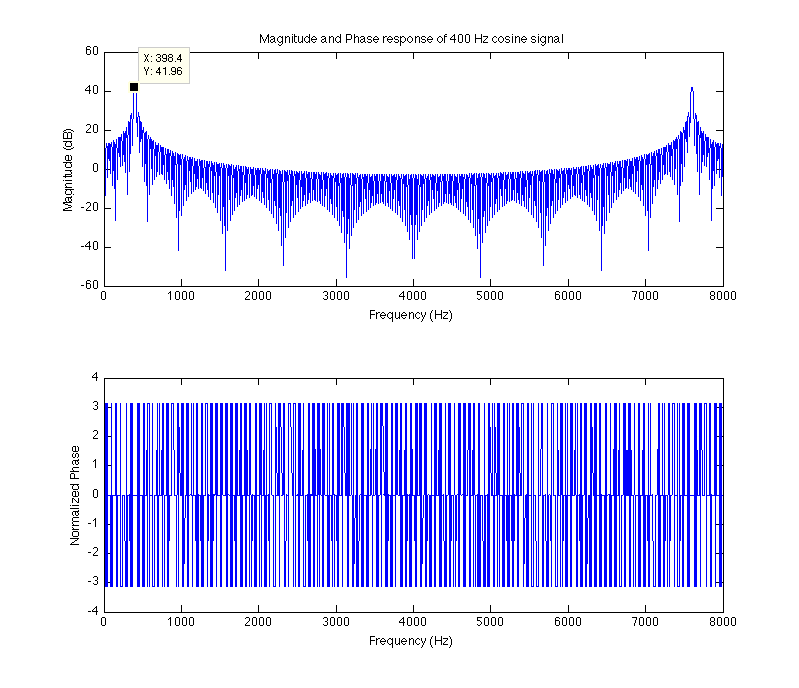
\includegraphics[scale=.7]{p1b}
\end{figure}

\emph{*Note that the graphical indication of the peak is found simply by the maximum sample, not through the parabolic interpolation, so it is not as accurate as the value returned in \emph{freqs}.}

\item  Matlab code for p1c.m:
\begin{verbatim}
[x fs] = wavread('s1.wav');
N = length(x);

Xlin = fft(x);

eps = .00000001;
Xwdb = 20*log10(abs(Xlin)+eps);

subplot(211);
plot([0: fs/N : fs - 1], Xwdb);
title('Magnitude and Phase response of 400 Hz cosine signal');
ylabel('Magnitude (dB)');
xlabel('Frequency (Hz)');
subplot(212);
plot([0: fs/N : fs - 1], angle(Xlin));
ylabel('Normalized Phase');
xlabel('Frequency (Hz)');

[peaks, freqs] = findpeaks(Xwdb,4,fs,boxcar(length(x)),length(x));

peaks
freqs
\end{verbatim}
The output of the above code is:
\begin{verbatim}
peaks = 1.0000    1.0000    1.0000
freqs = 1200         600        1800
\end{verbatim}
\newpage
and the plot looks like:
\begin{figure}[!h]
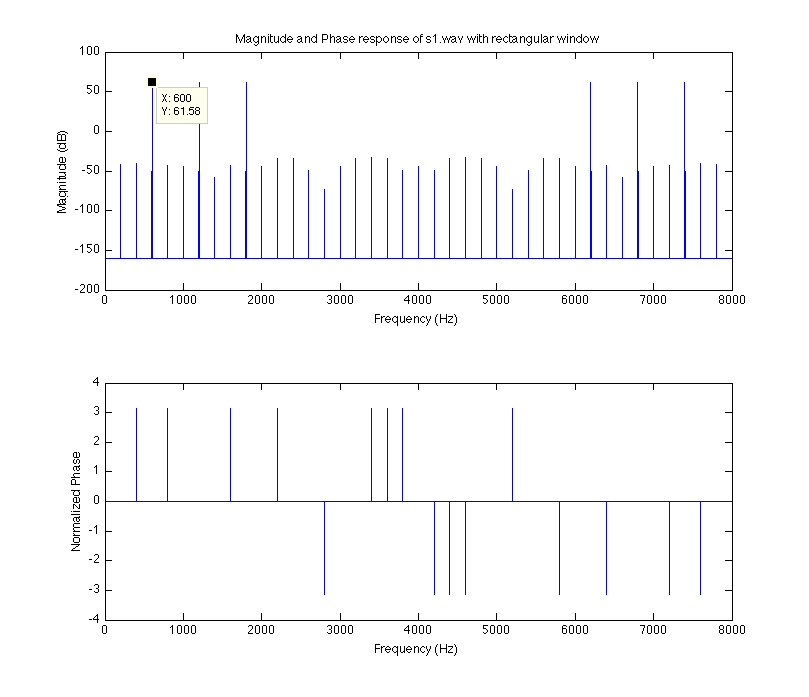
\includegraphics[scale=.7]{p1c}
\end{figure}

\newpage
\item Matlab code for p1d.m:
\begin{verbatim}
[x fs] = wavread('s1.wav');
N = length(x);

ham = hamming(length(x));
x_win = ham .* x;

Xlin = fft(x_win);

eps = .00000001;
Xwdb = 20*log10(abs(Xlin)+eps);

subplot(211);
plot([0: fs/N : fs - 1], Xwdb);
title('Magnitude and Phase response of s1.wav with Hamming window');
ylabel('Magnitude (dB)');
xlabel('Frequency (Hz)');
subplot(212);
plot([0: fs/N : fs - 1], angle(Xlin));
ylabel('Normalized Phase');
xlabel('Frequency (Hz)');

[peaks, freqs] = findpeaks(Xwdb, 4, fs, ham, length(Xwdb));

peaks
freqs
\end{verbatim}
The output of the above code is:
\begin{verbatim}
peaks = 1.0000    1.0000    1.0000
freqs = 1.0e+03 *
             1.2000    0.6000    1.8000
\end{verbatim}
\newpage
and the plot looks like:
\begin{figure}[!h]
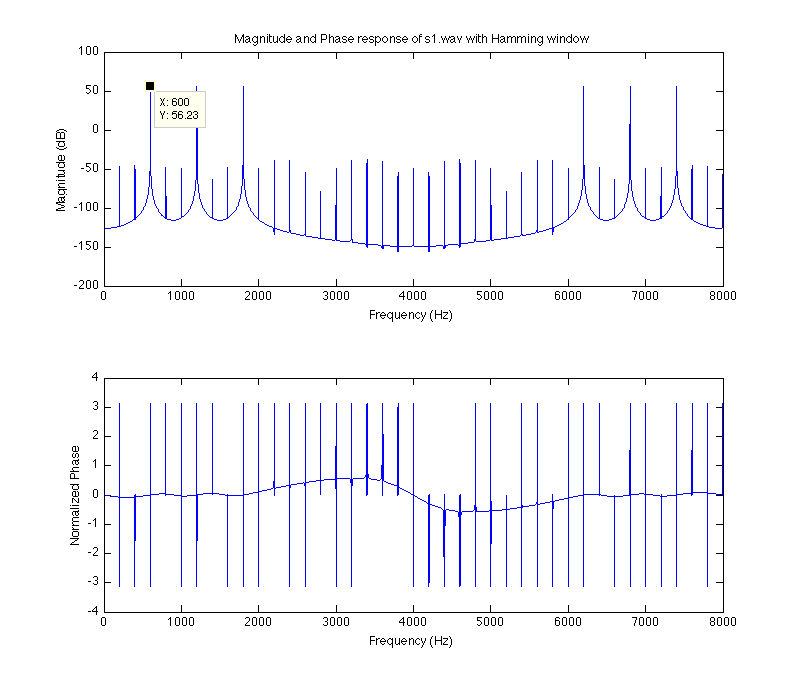
\includegraphics[scale=.7]{p1d}
\end{figure}
\end{enumerate}

\subsection*{Question 2}
\begin{enumerate}
\item \emph{(nothing to show)}
\item \emph{(nothing to show)}
\item The output of oboeanal is:
\begin{verbatim}
Read oboe.ff.C4B4.wav, fs = 44100.000000, nbits = 16, length = 29381,
samples = 0.7 sec
Estimated pitch = 260.710019 Hz
Nw = 2048
Nw =  4096
Nw = 8192
\end{verbatim}
\newpage
and the plot in \emph{Figure 1} looks like:
\begin{figure}[!h]
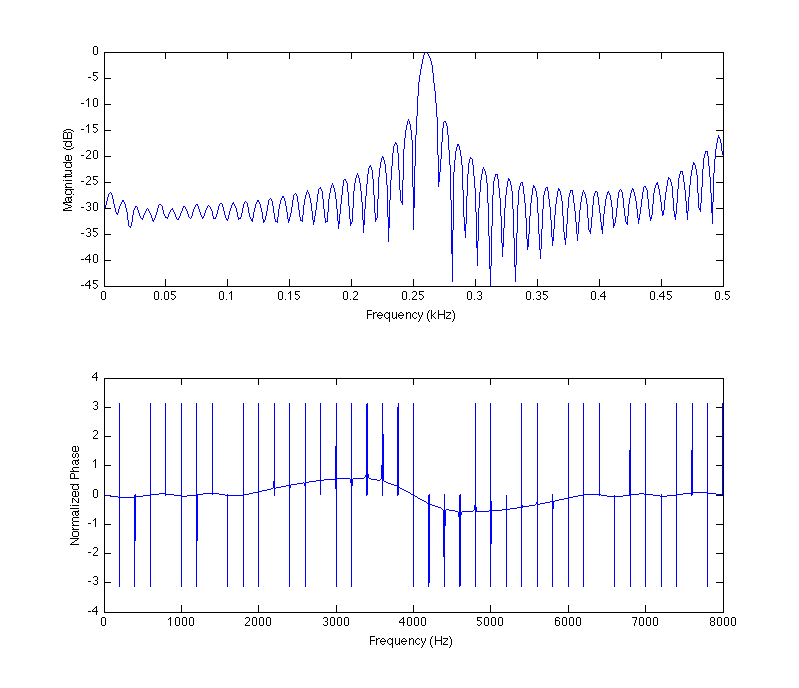
\includegraphics[scale=.7]{p2c}
\end{figure} \\
The frequency value at the peak magnitude lobe agrees exactly with the Estimated pitch of $260.71$.

\item All three windows show an ability to resolve the peaks, although the results clearly get better and better as the length of the window grows. By this I mean that the side lobes drop lower down and the noise floor gets lower, especially towards the higher frequencies.

\item The trend is that larger values of $K$ produce better, more resolvable results. Specifically, when $K=1$ the plot is very unclear, and the graph seems to indicate that the magnitude peaks are in the wrong order: it shows the third peak from the left as higher than the first and second peaks, as all the other graphs do.

\end{enumerate}


\end{document}
